\documentclass{amsart}

\usepackage[T1]{fontenc}
\usepackage[utf8]{inputenc}
\usepackage{amsmath,amssymb}
\usepackage{booktabs}
\usepackage[table]{xcolor}
\usepackage{array}
\usepackage{tikz}

\title{Atlas Tree Estimation Report}
\author{}
\date{}

\begin{document}

\maketitle

This report compares the stacking number and the tree estimation for every tree
in the NetworkX graph atlas with at least two vertices.

\medskip

During the generation of this report, the program checked for each atlas tree whether the stacking number is equal to the tree estimation. For all 24 trees considered here, the two values are equal.

\begin{center}
\setlength{\tabcolsep}{10pt}
\renewcommand{\arraystretch}{1.15}
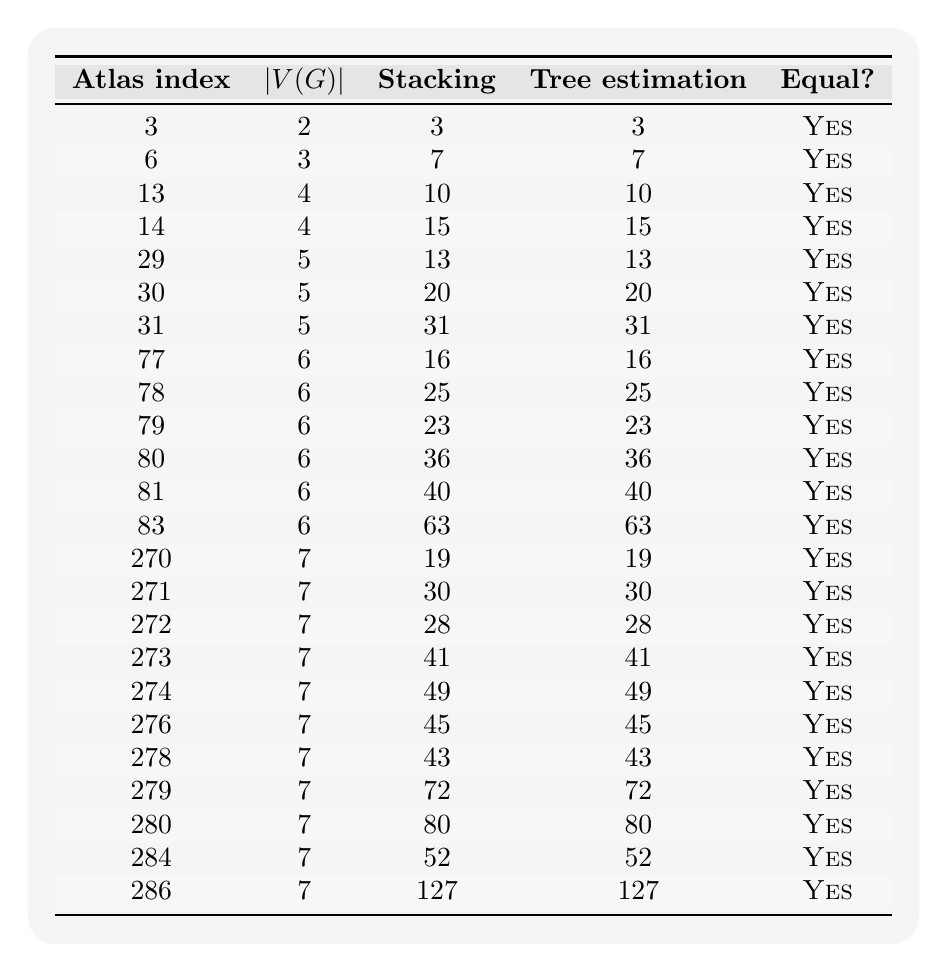
\begin{tikzpicture}
\node[rounded corners=10pt, fill=gray!8, inner sep=10pt] {
\begin{tabular}{ccccc}
\toprule
\rowcolor{gray!20}
\textbf{Atlas index} & \textbf{$|V(G)|$} & \textbf{Stacking} & \textbf{Tree estimation} & \textbf{Equal?} \\
\midrule
3 & 2 & 3 & 3 & \textsc{Yes} \\
\rowcolor{gray!6} 6 & 3 & 7 & 7 & \textsc{Yes} \\
13 & 4 & 10 & 10 & \textsc{Yes} \\
\rowcolor{gray!6} 14 & 4 & 15 & 15 & \textsc{Yes} \\
29 & 5 & 13 & 13 & \textsc{Yes} \\
\rowcolor{gray!6} 30 & 5 & 20 & 20 & \textsc{Yes} \\
31 & 5 & 31 & 31 & \textsc{Yes} \\
\rowcolor{gray!6} 77 & 6 & 16 & 16 & \textsc{Yes} \\
78 & 6 & 25 & 25 & \textsc{Yes} \\
\rowcolor{gray!6} 79 & 6 & 23 & 23 & \textsc{Yes} \\
80 & 6 & 36 & 36 & \textsc{Yes} \\
\rowcolor{gray!6} 81 & 6 & 40 & 40 & \textsc{Yes} \\
83 & 6 & 63 & 63 & \textsc{Yes} \\
\rowcolor{gray!6} 270 & 7 & 19 & 19 & \textsc{Yes} \\
271 & 7 & 30 & 30 & \textsc{Yes} \\
\rowcolor{gray!6} 272 & 7 & 28 & 28 & \textsc{Yes} \\
273 & 7 & 41 & 41 & \textsc{Yes} \\
\rowcolor{gray!6} 274 & 7 & 49 & 49 & \textsc{Yes} \\
276 & 7 & 45 & 45 & \textsc{Yes} \\
\rowcolor{gray!6} 278 & 7 & 43 & 43 & \textsc{Yes} \\
279 & 7 & 72 & 72 & \textsc{Yes} \\
\rowcolor{gray!6} 280 & 7 & 80 & 80 & \textsc{Yes} \\
284 & 7 & 52 & 52 & \textsc{Yes} \\
\rowcolor{gray!6} 286 & 7 & 127 & 127 & \textsc{Yes} \\
\bottomrule
\end{tabular}
};
\end{tikzpicture}
\end{center}

\end{document}
